% DoctIP Multi-Layered Zero-Trust Security Architecture
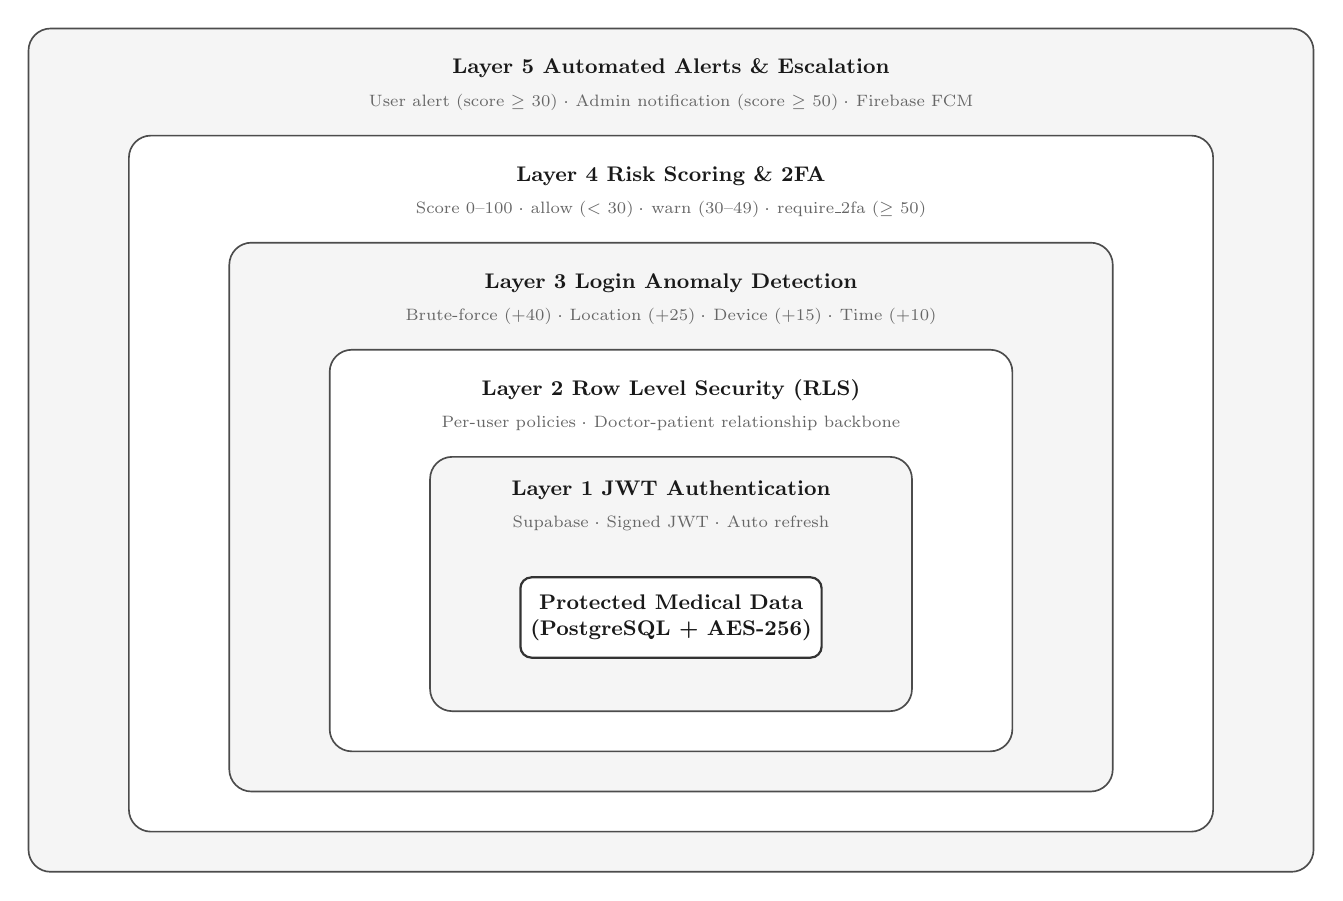
\begin{tikzpicture}[x=1cm,y=1cm, scale=0.85, every node/.style={scale=0.85}]
  \tikzset{
    layer/.style={draw=black!70, line width=0.6pt, rounded corners=8pt},
    lbl/.style={font=\small\bfseries, text=black!90},
    sub/.style={font=\scriptsize, text=black!60, text width=0.9*\boxwidth cm, align=center},
    core/.style={draw=black!80, fill=white, line width=0.8pt, rounded corners=4pt, font=\small\bfseries, align=center, minimum width=4.5cm, minimum height=1.2cm, text=black!90}
  }

  % Draw layers from outside in for proper overlapping
  
  % Layer 5
  \def\w{9.6} \def\boxwidth{19.2}
  \draw[layer, fill=black!4] (-\w, -4.8) rectangle (\w, 7.8);
  \node[lbl] at (0, 7.2) {Layer 5 Automated Alerts \& Escalation};
  \node[sub, text width=17cm] at (0, 6.7) {User alert (score\ $\geq$\ 30) \textperiodcentered{} Admin notification (score\ $\geq$\ 50) \textperiodcentered{} Firebase FCM};

  % Layer 4
  \def\w{8.1} \def\boxwidth{16.2}
  \draw[layer, fill=white] (-\w, -4.2) rectangle (\w, 6.2);
  \node[lbl] at (0, 5.6) {Layer 4 Risk Scoring \& 2FA};
  \node[sub, text width=15cm] at (0, 5.1) {Score 0--100 \textperiodcentered{} allow ($<$\ 30) \textperiodcentered{} warn (30--49) \textperiodcentered{} require\_2fa ($\geq$\ 50)};

  % Layer 3
  \def\w{6.6} \def\boxwidth{13.2}
  \draw[layer, fill=black!4] (-\w, -3.6) rectangle (\w, 4.6);
  \node[lbl] at (0, 4.0) {Layer 3 Login Anomaly Detection};
  \node[sub, text width=12cm] at (0, 3.5) {Brute-force (+40) \textperiodcentered{} Location (+25) \textperiodcentered{} Device (+15) \textperiodcentered{} Time (+10)};

  % Layer 2
  \def\w{5.1} \def\boxwidth{10.2}
  \draw[layer, fill=white] (-\w, -3.0) rectangle (\w, 3.0);
  \node[lbl] at (0, 2.4) {Layer 2 Row Level Security (RLS)};
  \node[sub, text width=9cm] at (0, 1.9) {Per-user policies \textperiodcentered{} Doctor-patient relationship backbone};

  % Layer 1
  \def\w{3.6} \def\boxwidth{7.2}
  \draw[layer, fill=black!4] (-\w, -2.4) rectangle (\w, 1.4);
  \node[lbl] at (0, 0.9) {Layer 1 JWT Authentication};
  \node[sub, text width=6cm] at (0, 0.4) {Supabase \textperiodcentered{} Signed JWT \textperiodcentered{} Auto refresh};

  % Core Data
  \node[core] at (0, -1.0) {Protected Medical Data\\(PostgreSQL + AES-256)};

\end{tikzpicture}

